\documentclass[12pt]{article}
% ============================================================================
% PACKAGE IMPORTS — FINAL, PUBLICATION-READY
% ============================================================================
% --- Geometry (load early) ---
\usepackage[margin=1in]{geometry}
\setlength{\headheight}{14pt}

% --- Math & Symbols ---
\usepackage{amsmath,amssymb}
\usepackage{siunitx}

% --- Tables ---
\usepackage{array}
\usepackage{booktabs}
\usepackage{multirow}

% --- Graphics & Figures ---
\usepackage{graphicx}
\usepackage{float}
\usepackage{caption}
\usepackage{subcaption}

% --- TikZ & PGFPlots ---
\usepackage{tikz}
\usetikzlibrary{shapes.geometric, arrows.meta, positioning, shadows, fit, calc, decorations.pathmorphing, shapes.symbols}
\usepackage{pgfplots}
\pgfplotsset{compat=1.18}

% --- Lists ---
\usepackage{enumitem}

% --- Colors & Boxes ---
\usepackage{xcolor}
\usepackage[framemethod=TikZ]{mdframed}

% --- Typography & Spacing ---
\usepackage{setspace}
\usepackage{lineno}

% --- Headers & Footers ---
\usepackage{fancyhdr}

% --- Bibliography ---
\usepackage[numbers,sort&compress]{natbib}

% --- Hyperlinks (load near end) ---
\usepackage[hidelinks]{hyperref}

% ============================================================================
% SIUNITX CONFIGURATION — FINAL, PUBLICATION-READY
% ============================================================================
\sisetup{
    range-phrase = --,
    range-units = single,
    detect-all,
    separate-uncertainty = true
}

% ============================================================================
% PAGE LAYOUT — FINAL, PUBLICATION-READY
% ============================================================================
\onehalfspacing
\setlength{\parindent}{15pt}
\setlength{\parskip}{6pt}

\pagestyle{fancy}
\fancyhf{}
\rhead{\small Hybrid mRNA Vaccine for Glioblastoma}
\rfoot{\thepage}
\renewcommand{\headrulewidth}{0.5pt}

% ============================================================================
% HYPERREF SETUP — FINAL, PUBLICATION-READY
% ============================================================================
\hypersetup{
    colorlinks=true,
    linkcolor=black,
    urlcolor=blue,
    citecolor=black,
    pdfauthor={Collin B. George},
    pdftitle={Hybrid mRNA Vaccine for Glioblastoma},
    pdfkeywords={glioblastoma, mRNA vaccine, blood-brain barrier, neoantigens, focused ultrasound, immunotherapy, IL-12, RIG-I ligands}
}

% ============================================================================
% TITLE AND AUTHOR INFORMATION — CORRECTED VERSION
% ============================================================================
\title{\textbf{A Translational Framework for a Hybrid mRNA Vaccine Targeting Glioblastoma:\\
Integrating Innate Priming, Personalized Neoantigens, and Blood--Brain Barrier Penetrating Delivery}}

\author{
\begin{minipage}{0.9\textwidth}
\centering
\textbf{Collin B. George, BS}\\[6pt]
\small University of Washington Medical Center, Seattle, WA, USA\\[4pt]
\small \texttt{cbg24@uw.edu}\\[4pt]
\small ORCID: \href{https://orcid.org/0009-0007-8162-6839}{0009-0007-8162-6839}\\[10pt]
\footnotesize\textit{This manuscript represents independent premedical research based on clinical}\\
\footnotesize\textit{observations at the Department of Anesthesiology and Pain Medicine.}\\
\footnotesize\textit{The views expressed are solely those of the author and do not represent UW Medicine.}
\end{minipage}
}

\date{}

% ============================================================================
% BEGIN DOCUMENT — FINAL, PUBLICATION-READY
% ============================================================================
\begin{document}

\maketitle
\thispagestyle{empty}

\newpage

% ============================================================================
% EDUCATIONAL DISCLAIMER PAGE — NEW ADDITION
% ============================================================================
\thispagestyle{empty}
\vspace*{3cm}
\begin{center}
\LARGE\textbf{Conceptual Translational Framework}\\[1cm]
\Large\textbf{Educational Synthesis Seeking Expert Validation}\\[2cm]

\normalsize
\begin{minipage}{0.85\textwidth}
\centering
This manuscript represents independent premedical research conducted through clinical observation rotations within the Department of Anesthesiology and Pain Medicine at the University of Washington Medical Center.

\vspace{0.5cm}

\textbf{Purpose:} To demonstrate translational reasoning skills and identify potential synergies across existing therapeutic modalities through systematic literature review.

\vspace{0.5cm}

\textbf{Limitations:} The author lacks direct experimental experience in GBM immunotherapy, mRNA vaccine development, or clinical trial design. This framework has not been validated through laboratory investigation or preclinical studies.

\vspace{0.5cm}

\textbf{Intended Use:} As a starting point for discussion with experienced researchers in neuro-oncology, immunotherapy, and biomedical engineering. The author seeks mentorship to evaluate scientific merit and refine concepts under expert guidance.

\vspace{0.5cm}

This work received no institutional funding and does not represent official positions of the University of Washington Medical Center or Pacific Northwest National Laboratory.

\vspace{0.5cm}

\textbf{Status:} Seeking faculty collaboration for potential development and validation.
\end{minipage}
\end{center}

\newpage

% ============================================================================
% ABSTRACT — REVISED WITH APPROPRIATE FRAMING
% ============================================================================
\begin{abstract}
Glioblastoma (GBM) remains lethal despite multimodal therapy, with median survival under 15 months. Immunotherapy has failed in over 100 clinical trials due to three fundamental barriers: inadequate immune priming in ``cold'' tumors, blood--brain barrier (BBB) exclusion of therapeutics, and profound local immunosuppression~\citep{lim2024,chen2024}.

Recent advances in mRNA vaccine technology, focused ultrasound-mediated BBB disruption, and checkpoint inhibition suggest potential synergies that could address these barriers simultaneously. This educational framework synthesizes evidence for integrating universal innate immune primers (poly(I:C)/RIG-I ligands, IL-12) with patient-specific neoantigen mRNA to activate dendritic cells and drive tumor-targeted T-cell responses~\citep{oloruntimehin2025,aunins2025}. BBB penetration could be achieved through peptide-modified lipid nanoparticles or focused ultrasound-guided delivery~\citep{han2025,chen2024fus}. Timed checkpoint blockade might exploit vaccine-induced PD-L1 upregulation to enhance infiltrating T-cell function.

Validation of such an approach would require stepwise progression: computational modeling to optimize dosing, in-vitro co-cultures to confirm antigen presentation, patient-derived xenografts to demonstrate BBB crossing and tumor control, and Phase I trials using post-resection focused ultrasound delivery with PET and ctDNA endpoints~\citep{karimi2024,sayour2024,manfredi2024}. Current manufacturing timelines of approximately 2--4 weeks from tumor sequencing to vaccine production could potentially align with surgical workflows~\citep{wang2025,hilf2024}.

\noindent\textbf{Significance:} This synthesis identifies potential mechanistic synergies across existing therapeutic modalities. Translation to clinical application would require institutional partnerships, preclinical validation, and expert guidance from established researchers in neuro-oncology and immunotherapy. The framework is presented for evaluation of scientific merit and potential refinement under faculty mentorship.

\noindent\textbf{Author's Note:} This work represents educational exploration of translational concepts rather than a validated research protocol. The author recognizes substantial gaps between literature synthesis and clinical implementation, and seeks collaboration with experienced investigators to assess feasibility.
\end{abstract}

\noindent\textbf{Keywords:} glioblastoma; mRNA vaccine; blood-brain barrier; neoantigens; focused ultrasound; immunotherapy; IL-12; RIG-I ligands

\newpage

% ============================================================================
% INTRODUCTION — REFRAMED WITH APPROPRIATE HUMILITY
% ============================================================================
\section{Introduction}

\subsection{The GBM Treatment Crisis}
Glioblastoma (GBM) kills nearly all patients within two years of diagnosis. Despite maximal surgical resection, radiotherapy, and temozolomide chemotherapy, median overall survival remains approximately 15 months~\citep{lim2024}. The tumor's rapid proliferation, diffuse infiltration, and profound heterogeneity drive this recalcitrance, but a deeper problem has emerged: GBM actively suppresses the immune system.

Over 100 immunotherapy trials have failed in GBM, including multiple Phase III checkpoint inhibitor studies~\citep{chen2024,reardon2020}. CheckMate-143 and CheckMate-498 showed no survival benefit from nivolumab versus standard care, revealing that GBM is fundamentally different from immunotherapy-responsive cancers like melanoma or lung cancer. The tumor is immunologically ``cold''—characterized by low tumor mutation burden (typically $<$10 mutations/Mb), sparse T-cell infiltration, and a microenvironment dominated by immunosuppressive myeloid-derived suppressor cells, regulatory T cells, and M2-polarized macrophages~\citep{liau2023}.

\subsection{Three Fundamental Barriers}
Current evidence suggests GBM's resistance to immunotherapy stems from three interconnected barriers.

First, inadequate immune priming: the tumor generates few neoantigens and lacks ``danger'' signals that normally recruit and activate dendritic cells. Without proper antigen presentation, the adaptive immune system never recognizes GBM as foreign.

Second, the blood--brain barrier (BBB) physically excludes systemic therapeutics, including large-molecule vaccines and immune effectors. While BBB disruption occurs focally due to tumor neovascularization, this permeability is heterogeneous and may be insufficient for consistent drug delivery~\citep{lim2024}. The brain's immune-privileged status further limits antigen presentation and lymphatic drainage.

Third, profound local immunosuppression: even when T cells infiltrate, they encounter hypoxia, necrosis, and cytokine gradients that favor exhaustion and tolerance rather than tumor killing.

\subsection{Potential for Hybrid mRNA Vaccine Approaches}
Personalized neoantigen vaccines have shown promise in other solid tumors, eliciting robust CD8$^+$ T-cell responses in early-phase trials~\citep{hilf2024}. mRNA platforms, validated by COVID-19 vaccine success, enable rapid production with inherent adjuvancy through lipid nanoparticle (LNP) delivery~\citep{oloruntimehin2025}. However, single-modality approaches may fail in GBM because they address only one barrier at a time.

Recent literature suggests potential for integrating three innovations simultaneously. First, universal innate immune primers (encoded as mRNA or co-formulated) could mimic viral infection to activate dendritic cells and recruit effectors, potentially converting cold tumors hot. Second, patient-specific neoantigen mRNA might drive tumor-targeted T-cell expansion. Third, BBB-penetrating delivery—through peptide-modified LNPs or focused ultrasound—could enable intratumoral access. Timed checkpoint blockade might then release vaccine-primed T cells from local suppression.

This conceptual framework builds on clinical advances from 2024--2025, including IL-12 mRNA-LNPs that suppressed tumors in preclinical models~\citep{aunins2025,tapescu2024} and focused ultrasound achieving BBB opening enhancement in human trials~\citep{manfredi2024,chen2024fus}. Manufacturing timelines of 2--4 weeks from tumor sequencing to GMP-grade vaccine production have been reported in recent studies, though practical implementation challenges remain substantial~\citep{wang2025,hilf2024}.

\subsection{Framework Scope and Limitations}

\textbf{What this framework represents:} An educational synthesis examining potential mechanistic synergies across existing therapeutic modalities (mRNA vaccines, focused ultrasound, checkpoint inhibition) through systematic literature review. The integration proposed draws from published preclinical and early clinical studies but has not been validated experimentally.

\textbf{What this framework does NOT represent:} 
\begin{itemize}[leftmargin=*,noitemsep]
\item A validated research protocol ready for clinical implementation
\item Primary research or experimental data
\item Clinical guidance for GBM treatment
\item A complete drug development plan with regulatory pathway
\end{itemize}

\textbf{Author's perspective:} As a premedical trainee with laboratory experience but lacking direct expertise in GBM immunotherapy, mRNA vaccine development, or clinical trial design, this synthesis identifies potential opportunities for integration that would require validation by multidisciplinary teams with domain expertise. Practical constraints evident to experienced practitioners may not be fully captured in this literature-based analysis.

\textbf{Intended purpose:} To demonstrate translational reasoning skills, identify potential research questions, and serve as a starting point for discussion with faculty researchers in neuro-oncology, immunology, and biomedical engineering. The author seeks mentorship to evaluate whether the proposed integration has scientific merit and, if so, to refine concepts under expert guidance.

\subsection{Paper Organization}
This framework outlines potential vaccine mechanisms (Section 2), safety and dosing considerations that would need to be addressed through computational modeling and preclinical work (Section 3), a hypothetical validation roadmap from in-silico to Phase I (Section 4), and discussion of limitations and knowledge gaps (Section 5). The goal is to present concepts for expert evaluation rather than to provide definitive solutions.

% ============================================================================
% MECHANISM OF ACTION — REFRAMED AS POTENTIAL APPROACH
% ============================================================================
\section{Potential Mechanism of Action}

Recent literature suggests that a hybrid vaccine approach could operate through three integrated arms working synergistically to address GBM's immunoresistance (Figure~\ref{fig:mechanism}). The following sections describe potential mechanisms based on published preclinical and clinical studies.

\subsection{Innate Priming: Potential for Immune Activation}
The innate priming component could include synthetic polyinosinic:polycytidylic acid [poly(I:C)] co-formulated with mRNA encoding retinoic acid-inducible gene I (RIG-I) ligands and interleukin-12 (IL-12)~\citep{ammi2015,jiang2023,aunins2025}. When delivered in LNPs, these agents trigger pattern recognition receptors in antigen-presenting cells, particularly dendritic cells, as demonstrated in preclinical models.

The cascade mimics viral infection. Poly(I:C) and RIG-I ligands activate endosomal sensors, inducing controlled type I interferon (IFN-$\alpha$/$\beta$) production. This drives dendritic cell maturation, upregulates co-stimulatory molecules (CD80/86), and triggers chemokine release (CXCL10, CCL5) that recruits natural killer cells and macrophages to the tumor site~\citep{jiang2023}.

IL-12 could amplify this response by polarizing toward Th1 immunity. It enhances cytotoxic T lymphocyte differentiation while suppressing regulatory T cells, creating a pro-inflammatory environment that might counter GBM's baseline immunosuppression~\citep{aunins2025,tapescu2024}. Critically, mRNA expression is transient—typically 24--72 hours—providing a pulse of activation without chronic inflammation.

Preclinical validation supports this approach. IL-12 mRNA-LNPs suppressed tumor growth in orthotopic GBM models through NK and CTL recruitment, achieving tumor regression without dose-limiting toxicities at intratumoral doses up to 12~$\mu$g~\citep{aunins2025,lai2018}. However, translation to human GBM would require careful dose-finding studies and safety monitoring.

\subsection{Adaptive Targeting: Personalized Neoantigen Recognition}
The adaptive arm could encode patient-specific neoantigens identified through tumor exome and transcriptome sequencing. Bioinformatic pipelines (e.g., NetMHCpan) predict high-affinity epitopes for MHC class I presentation, prioritizing mutations likely to elicit CD8$^+$ T-cell responses~\citep{hilf2024}.

When LNPs deliver neoantigen mRNA to dendritic cells, the encoded proteins are synthesized endogenously, processed through the proteasome, and loaded onto MHC-I molecules. This endogenous presentation pathway is critical—it mimics viral infection and efficiently primes CD8$^+$ T cells without requiring exogenous protein uptake.

The anticipated result would be clonal expansion of tumor-specific effector-memory T cells capable of trafficking to the CNS and recognizing GBM cells expressing the target mutations. Multi-epitope designs (typically 5--15 neoantigens per vaccine, constrained by GBM's low mutation burden) could provide redundancy against tumor escape through antigen loss~\citep{wang2025,hilf2024}.

\textbf{Important caveat:} GBM's low mutational burden (typically $<$10 mutations/Mb) presents a significant challenge. Unlike melanoma or lung cancer where 20+ high-quality neoantigens are often available, GBM patients may yield only 5--10 suitable epitopes after filtering for MHC binding, expression level, and clonality. Some patients may have insufficient neoantigens for a purely personalized approach, potentially requiring supplementation with tumor-associated antigens like EGFRvIII or IL-13R$\alpha$2.

\subsection{Synergistic Integration}
Co-encapsulating innate primers and neoantigens in the same LNP formulation could ensure spatiotemporal coordination. Innate signals would amplify antigen processing by increasing epitope density on dendritic cells, enhance T-cell receptor avidity through sustained co-stimulation, and create a cytokine milieu (IFN-$\gamma$, IL-12) that promotes effector rather than regulatory differentiation~\citep{oloruntimehin2025}.

This design mirrors successful pathogen responses: the innate arm provides the ``adjuvant'' context that signals neoantigens are dangerous, while the adaptive arm provides specificity. However, the actual magnitude of synergy in GBM remains to be determined experimentally.

\subsection{BBB Penetration Strategies}
Delivering this vaccine payload to GBM requires overcoming the BBB. Two complementary approaches have shown promise in recent literature (Figure~\ref{fig:bbb}).

\textbf{Peptide-Modified LNPs:} Conjugating targeting peptides to LNP surfaces could enable receptor-mediated transcytosis. Rabies virus glycoprotein (RVG) peptide binds nicotinic acetylcholine receptors on brain endothelium, achieving approximately 10-fold increased brain uptake in rodent models~\citep{han2025}. Transferrin receptor (TfR) targeting leverages natural iron transport, with clinical precedent in antibody--drug conjugates. These modifications maintain LNP stability and can be administered systemically.

\textbf{Critical limitation:} The 10-fold enhancement reported for RVG-modified LNPs comes from rodent studies with ideal conditions. Human translation faces significant challenges: receptor expression varies across patients, BBB disruption in GBM is heterogeneous, and large LNPs (~100 nm) may achieve lower enhancement than the small molecules tested in many studies. Clinical validation of peptide-LNP brain delivery in humans is still limited.

\textbf{Focused Ultrasound (FUS):} Transcranial FUS with microbubbles transiently opens the BBB through acoustic cavitation, creating reversible sonoporation without permanent damage. MRI guidance provides millimeter-scale spatial precision, enabling focal delivery to resection cavities. Human trials in GBM have demonstrated safety, with transient mild headaches in $<$10\% of patients and gadolinium MRI confirming BBB opening~\citep{shen2024,manfredi2024}. 

\textbf{Important nuance on enhancement:} Published reports describe FUS achieving "up to 50-fold" BBB enhancement, but this figure requires context. The 50-fold enhancement typically refers to small molecules in highly controlled preclinical conditions. For large therapeutic payloads like mRNA-LNPs (~100 nm), enhancement is more variable and may range from 2--10 fold in human applications, depending on molecular weight, tumor vasculature heterogeneity, and patient-specific factors~\citep{chen2024fus,meng2020}. BBB closure occurs within 24--48 hours, requiring careful timing of therapeutic administration.

\textbf{Practical constraints:} FUS requires specialized equipment not widely available, MRI-compatible operating rooms or dedicated suites, and operator expertise. Multiple treatment sessions may be needed, each requiring careful monitoring for potential complications like vasogenic edema or petechial hemorrhage (though these have been rare and generally asymptomatic in clinical trials).

\begin{figure}[!htbp]
\centering
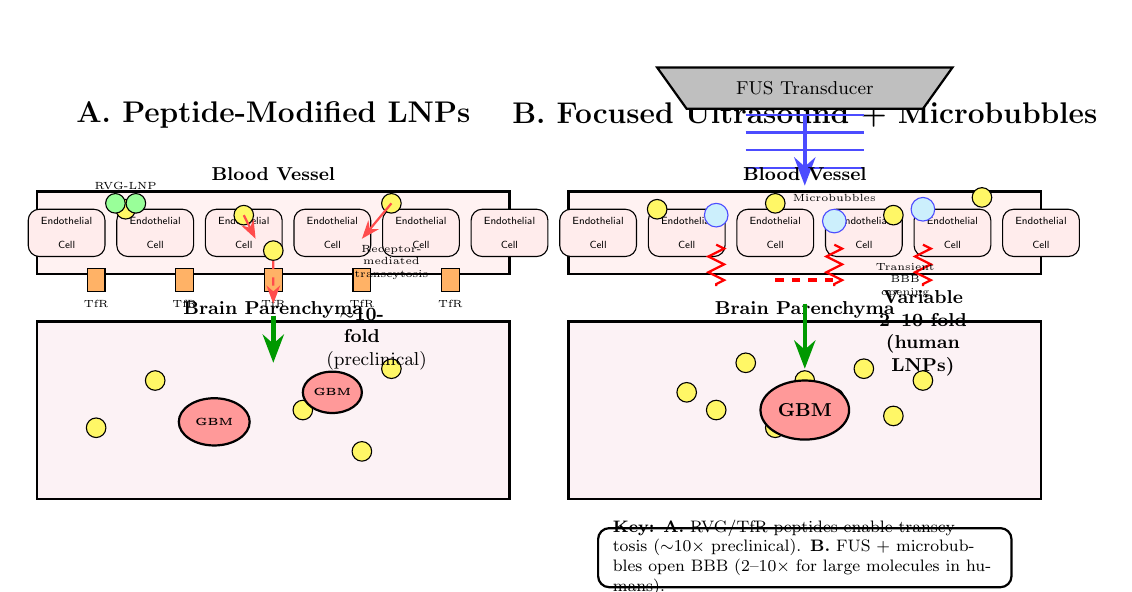
\begin{tikzpicture}[
    font=\sffamily,
    scale=0.75,
    every node/.style={transform shape},
    % Node styles
    cell/.style={rectangle, draw, rounded corners, minimum width=2cm, minimum height=0.8cm, align=center, fill=blue!10},
    vessel/.style={rectangle, draw, thick, minimum width=8cm, minimum height=1.5cm, fill=red!5},
    brain/.style={rectangle, draw, thick, minimum width=8cm, minimum height=3cm, fill=purple!5},
    lnp/.style={circle, draw, fill=yellow!60, minimum size=0.3cm},
    peptide/.style={draw, fill=green!40, minimum size=0.25cm, circle},
    receptor/.style={rectangle, draw, fill=orange!60, minimum width=0.3cm, minimum height=0.5cm, rounded corners},
    microbubble/.style={circle, draw=blue!70, fill=cyan!20, minimum size=0.4cm},
    arrow/.style={-Stealth, thick, color=red!70},
]

% ============================================================================
% LEFT PANEL: PEPTIDE-MODIFIED LNPs
% ============================================================================
\node[font=\Large\bfseries] at (-4.5, 7.5) {A. Peptide-Modified LNPs};

% Blood vessel (top)
\draw[thick, fill=red!5] (-8.5, 4.8) rectangle (-0.5, 6.2);
\node[font=\small\bfseries] at (-4.5, 6.5) {Blood Vessel};

% Endothelial cells layer
\foreach \x in {-8, -6.5, -5, -3.5, -2, -0.5} {
    \node[cell, minimum width=1.3cm, fill=pink!30] at (\x, 5.5) {\tiny Endothelial\\\tiny Cell};
}

% Receptors on endothelial cells
\foreach \x in {-7.5, -6, -4.5, -3, -1.5} {
    \draw[fill=orange!60, draw=black] (\x-0.15, 4.5) rectangle (\x+0.15, 4.9);
    \node[font=\tiny] at (\x, 4.3) {TfR};
}

% Peptide-modified LNPs in blood
\node[lnp] (lnp1) at (-7, 5.9) {};
\foreach \angle in {30, 150} {
    \node[peptide, minimum size=0.12cm] at ([shift=(\angle:0.2cm)]lnp1) {};
}
\node[font=\tiny] at (-7, 6.3) {RVG-LNP};

\node[lnp] at (-5, 5.8) {};
\node[lnp] at (-2.5, 6) {};

% Transcytosis process
\node[lnp] (lnp4) at (-4.5, 5.2) {};
\draw[arrow, dashed] (lnp4) -- (-4.5, 4.3);
\node[font=\tiny, text width=1.5cm, align=center] at (-2.5, 5) {Receptor-\\mediated\\transcytosis};

% Brain parenchyma (bottom)
\draw[thick, fill=purple!5] (-8.5, 1) rectangle (-0.5, 4);
\node[font=\small\bfseries] at (-4.5, 4.2) {Brain Parenchyma};

% LNPs delivered to brain
\foreach \pos in {(-6.5, 3), (-4, 2.5), (-2.5, 3.2), (-7.5, 2.2), (-3, 1.8)} {
    \node[lnp] at \pos {};
}

% GBM tumor cells
\draw[fill=red!40, draw=black, thick] (-5.5, 2.3) ellipse (0.6cm and 0.4cm);
\node[font=\tiny\bfseries] at (-5.5, 2.3) {GBM};
\draw[fill=red!40, draw=black, thick] (-3.5, 2.8) ellipse (0.5cm and 0.35cm);
\node[font=\tiny\bfseries] at (-3.5, 2.8) {GBM};

% Arrows showing delivery
\draw[arrow] (-5, 5.8) -- (-4.8, 5.4);
\draw[arrow] (-2.5, 6) -- (-3, 5.4);
\draw[arrow, green!60!black, ultra thick] (-4.5, 4.1) -- (-4.5, 3.3);
\node[font=\small, text width=1.2cm, align=center] at (-3, 3.7) {\textbf{$\sim$10-fold}\\(preclinical)};

% ============================================================================
% RIGHT PANEL: FOCUSED ULTRASOUND
% ============================================================================
\node[font=\Large\bfseries] at (4.5, 7.5) {B. Focused Ultrasound + Microbubbles};

% Ultrasound transducer
\draw[fill=gray!50, draw=black, thick] (2, 8.3) -- (7, 8.3) -- (6.5, 7.6) -- (2.5, 7.6) -- cycle;
\node[font=\small] at (4.5, 7.95) {FUS Transducer};

% Ultrasound waves (simple lines)
\foreach \y in {7.5, 7.2, 6.9, 6.6} {
    \draw[blue!70, thick] (3.5, \y) -- (5.5, \y);
}
\draw[blue!70, ultra thick, -Stealth] (4.5, 7.5) -- (4.5, 6.3);

% Blood vessel (top)
\draw[thick, fill=red!5] (0.5, 4.8) rectangle (8.5, 6.2);
\node[font=\small\bfseries] at (4.5, 6.5) {Blood Vessel};

% Endothelial cells layer
\foreach \x in {1, 2.5, 4, 5.5, 7, 8.5} {
    \node[cell, minimum width=1.3cm, fill=pink!30] at (\x, 5.5) {\tiny Endothelial\\\tiny Cell};
}

% Microbubbles
\foreach \pos in {(3, 5.8), (5, 5.7), (6.5, 5.9)} {
    \node[microbubble] at \pos {};
}
\node[font=\tiny] at (5, 6.1) {Microbubbles};

% Cavitation effects (zigzag lines)
\foreach \x in {3, 5, 6.5} {
    \draw[red, thick, decorate, decoration={zigzag, segment length=2mm, amplitude=1mm}] (\x, 5.3) -- (\x, 4.6);
}

% Disrupted tight junctions
\draw[red, ultra thick, dashed] (4, 4.7) -- (5, 4.7);
\node[font=\tiny, text width=1.2cm, align=center] at (6.2, 4.7) {Transient\\BBB\\opening};

% Regular LNPs in blood
\foreach \pos in {(2, 5.9), (4, 6), (6, 5.8), (7.5, 6.1)} {
    \node[lnp] at \pos {};
}

% Brain parenchyma (bottom)
\draw[thick, fill=purple!5] (0.5, 1) rectangle (8.5, 4);
\node[font=\small\bfseries] at (4.5, 4.2) {Brain Parenchyma};

% LNPs delivered to brain (more concentrated)
\foreach \pos in {(3.5, 3.3), (4.5, 3), (5.5, 3.2), (3, 2.5), (4, 2.2), (5, 2.7), (6, 2.4), (2.5, 2.8), (6.5, 3)} {
    \node[lnp] at \pos {};
}

% GBM tumor cells
\draw[fill=red!40, draw=black, thick] (4.5, 2.5) ellipse (0.75cm and 0.5cm);
\node[font=\small\bfseries] at (4.5, 2.5) {GBM};

% Arrows showing enhanced delivery
\draw[arrow, green!60!black, ultra thick] (4.5, 4.3) -- (4.5, 3.2);
\node[font=\small\bfseries, text width=2cm, align=center] at (6.5, 3.8) {Variable\\2--10-fold\\(human LNPs)};

% Legend box
\draw[thick, rounded corners, fill=white] (1, -0.5) rectangle (8, 0.5);
\node[font=\footnotesize, text width=6.5cm, align=left] at (4.5, 0) {
\textbf{Key:} \textbf{A.} RVG/TfR peptides enable transcytosis ($\sim$10$\times$ preclinical).
\textbf{B.} FUS + microbubbles open BBB (2--10$\times$ for large molecules in humans).
};

\end{tikzpicture}
\caption{Comparative blood-brain barrier penetration strategies using peptide-modified LNPs and focused ultrasound with microbubbles. \textbf{(A)} Peptide-modified lipid nanoparticles (LNPs) conjugated with RVG or TfR-targeting peptides undergo receptor-mediated transcytosis across brain endothelium, achieving approximately 10-fold enhancement in preclinical models. Human translation requires validation. \textbf{(B)} Focused ultrasound (FUS) with systemically administered microbubbles creates transient, reversible BBB opening through acoustic cavitation. Enhancement for large therapeutic molecules like LNPs in human applications is variable (typically 2--10-fold) depending on molecular characteristics and patient-specific factors. Both approaches require further clinical validation in GBM populations.}
\label{fig:bbb}
\end{figure}

\subsection{Checkpoint Blockade Integration}
The vaccine approach could be designed to synergize with anti-PD-1 therapy. Vaccine-induced activation upregulates PD-L1 on tumor cells and APCs---a resistance mechanism that checkpoint inhibitors might exploit~\citep{chen2024}.

Timing would be critical. Anti-PD-1 administration could begin 1--2 weeks post-vaccination, when T-cell infiltration might peak but before exhaustion sets in. This could potentially convert checkpoint blockade from ineffective monotherapy (as seen in CheckMate trials) to a strategy that releases vaccine-primed, tumor-specific T cells.

\textbf{Important caveat:} The optimal timing of checkpoint inhibition relative to vaccination remains uncertain in GBM. The 1--2 week interval is extrapolated from other tumor types and preclinical models. GBM's unique immunosuppressive microenvironment and BBB considerations may require different timing strategies that would need to be determined empirically through clinical trials.

This mechanistic framework suggests a self-sustaining loop: innate priming recruits and activates APCs, neoantigen presentation drives clonal T-cell expansion, BBB-penetrating delivery ensures intratumoral access, and checkpoint blockade maintains effector function. However, the actual efficacy of this integrated approach in human GBM patients remains to be established through rigorous preclinical and clinical investigation.

\begin{figure}[!htbp]
\centering
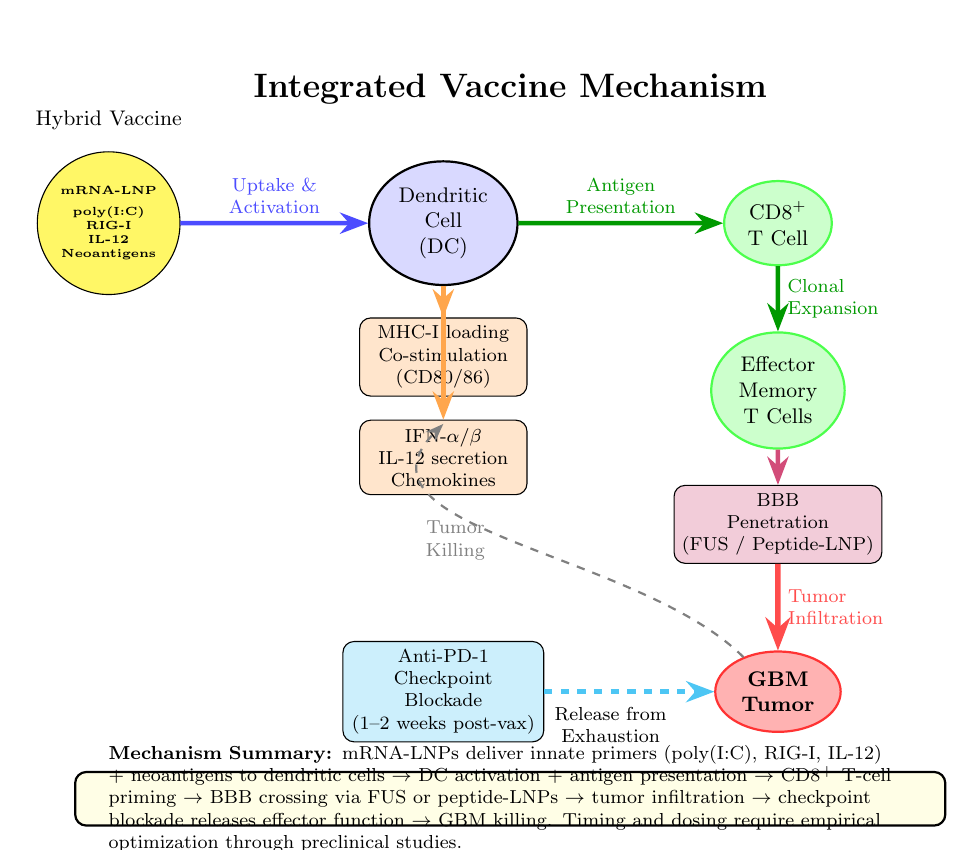
\begin{tikzpicture}[
    font=\sffamily,
    scale=0.85,
    every node/.style={transform shape},
    % Node styles
    lnp/.style={circle, draw=black, fill=yellow!60, minimum size=1.2cm, align=center, font=\tiny\bfseries},
    cell/.style={ellipse, draw=black, thick, minimum width=2cm, minimum height=1.2cm, align=center, fill=blue!15, font=\small},
    tumor/.style={ellipse, draw=red!80, thick, fill=red!30, minimum width=1.8cm, minimum height=1.2cm, align=center, font=\small\bfseries},
    tcell/.style={ellipse, draw=green!70, thick, fill=green!20, minimum width=1.5cm, minimum height=1cm, align=center, font=\small},
    arrow/.style={-Stealth, ultra thick},
    process/.style={rectangle, draw, rounded corners, fill=orange!20, minimum width=2.5cm, minimum height=0.9cm, align=center, font=\footnotesize},
]

% Title
\node[font=\Large\bfseries] at (0, 8) {Integrated Vaccine Mechanism};

% Step 1: LNP with components
\node[lnp] (lnp) at (-6, 6) {mRNA-LNP\\[0.1cm]poly(I:C)\\RIG-I\\IL-12\\Neoantigens};
\node[font=\small, above=0.2cm of lnp] {Hybrid Vaccine};

% Step 2: Dendritic Cell
\node[cell] (dc) at (-1, 6) {Dendritic\\Cell\\(DC)};

% Arrow 1: LNP to DC
\draw[arrow, blue!70] (lnp) -- (dc) node[midway, above, font=\footnotesize, text width=2cm, align=center] {Uptake \&\\Activation};

% Step 3: DC processes
\node[process] (process1) at (-1, 4) {MHC-I loading\\Co-stimulation\\(CD80/86)};
\node[process] (process2) at (-1, 2.5) {IFN-$\alpha$/$\beta$\\IL-12 secretion\\Chemokines};

% Arrows from DC to processes
\draw[arrow, orange!70] (dc) -- (process1);
\draw[arrow, orange!70] (dc) -- (process2);

% Step 4: T Cell Activation
\node[tcell] (tcell) at (4, 6) {CD8$^+$\\T Cell};

% Arrow: DC to T cell
\draw[arrow, green!60!black] (dc) -- (tcell) node[midway, above, font=\footnotesize, text width=2cm, align=center] {Antigen\\Presentation};

% Step 5: T Cell Expansion
\node[tcell] (tcell_expanded) at (4, 3.5) {Effector\\Memory\\T Cells};
\draw[arrow, green!60!black] (tcell) -- (tcell_expanded) node[midway, right, font=\footnotesize, text width=1.5cm, align=left] {Clonal\\Expansion};

% Step 6: BBB Crossing
\node[process, fill=purple!20] (bbb) at (4, 1.5) {BBB\\Penetration\\(FUS / Peptide-LNP)};
\draw[arrow, purple!70] (tcell_expanded) -- (bbb);

% Step 7: Tumor
\node[tumor] (tumor) at (4, -1) {GBM\\Tumor};

% Arrow: T cells to tumor
\draw[arrow, red!70, line width=2pt] (bbb) -- (tumor) node[midway, right, font=\footnotesize, text width=1.8cm, align=left] {Tumor\\Infiltration};

% Step 8: Checkpoint Blockade
\node[process, fill=cyan!20, minimum width=3cm] (checkpoint) at (-1, -1) {Anti-PD-1\\Checkpoint\\Blockade\\(1--2 weeks post-vax)};

% Arrow: checkpoint to tumor interaction
\draw[arrow, cyan!70, dashed] (checkpoint) to[out=0, in=180] (tumor);
\node[font=\footnotesize, text width=2cm, align=center] at (1.5, -1.5) {Release from\\Exhaustion};

% Feedback arrow
\draw[arrow, dashed, gray, thick] (tumor) to[out=135, in=225] node[midway, left, font=\footnotesize, text width=1.5cm, align=center] {Tumor\\Killing} (-1, 3);

% Legend/Notes box
\draw[thick, rounded corners, fill=yellow!10] (-6.5, -3) rectangle (6.5, -2.2);
\node[font=\footnotesize, text width=12cm, align=left] at (0, -2.6) {
\textbf{Mechanism Summary:} mRNA-LNPs deliver innate primers (poly(I:C), RIG-I, IL-12) + neoantigens to dendritic cells $\rightarrow$ DC activation + antigen presentation $\rightarrow$ CD8$^+$ T-cell priming $\rightarrow$ BBB crossing via FUS or peptide-LNPs $\rightarrow$ tumor infiltration $\rightarrow$ checkpoint blockade releases effector function $\rightarrow$ GBM killing. Timing and dosing require empirical optimization through preclinical studies.
};

\end{tikzpicture}
\caption{Proposed integrated mechanism of hybrid mRNA vaccine for GBM immunotherapy. The vaccine combines innate immune primers (poly(I:C), RIG-I ligands, IL-12 mRNA) with patient-specific neoantigen mRNA in lipid nanoparticles. Dendritic cell uptake triggers activation, antigen processing, and MHC-I presentation to prime CD8$^+$ T cells. BBB penetration via focused ultrasound or peptide-modified LNPs enables tumor infiltration. Timed checkpoint blockade (1--2 weeks post-vaccination) could potentially sustain effector function against local immunosuppression. This framework represents a conceptual synthesis requiring experimental validation across each mechanistic step.}
\label{fig:mechanism}
\end{figure}

% ============================================================================
% SAFETY AND DOSING CONSIDERATIONS — REFRAMED
% ============================================================================
\section{Safety and Dosing Considerations}

Translation of this conceptual framework to clinical application would require extensive safety assessment and dose optimization studies. The following sections outline potential safety considerations based on published literature, recognizing that actual human dosing would need to be determined through systematic preclinical and Phase I trials.

\subsection{Component-Specific Safety Profiles}
Each vaccine component has distinct safety considerations derived from published clinical and preclinical studies.

\subsubsection{Poly(I:C) and RIG-I Ligands}
Poly(I:C) has been tested in cancer vaccine trials at doses of 1--20~mg systemically, with dose-limiting toxicities including flu-like symptoms, transient transaminase elevation, and hypotension at higher doses~\citep{ammi2015}. When formulated in LNPs for local delivery, doses may be substantially lower (estimated 100--500~$\mu$g range based on preclinical studies), potentially reducing systemic toxicity while maintaining local adjuvant effects.

RIG-I ligands have shown promising safety in early trials when delivered as naked RNA oligonucleotides. Type I interferon induction is self-limiting due to negative feedback loops, though monitoring for autoimmune activation would be prudent given the pathway's role in lupus and other inflammatory conditions~\citep{jiang2023}.

\textbf{Proposed safety threshold (requiring validation):} Combined poly(I:C) + RIG-I ligand doses should potentially remain below levels that trigger systemic IFN-$\alpha$ concentrations $>$100 pg/mL (associated with flu-like symptoms) while achieving local concentrations sufficient for DC activation. This threshold would need to be established through dose-escalation studies.

\subsubsection{IL-12 mRNA}
IL-12 has a narrow therapeutic window. Systemic recombinant IL-12 protein caused severe toxicities in 1990s trials, including hepatotoxicity, hematologic suppression, and fatal outcomes at doses exceeding 500~ng/kg/week~\citep{lai2018}. However, mRNA delivery offers potential advantages: transient local expression (24--72h), lower peak concentrations compared to protein bolus, and LNP-mediated tissue targeting.

Preclinical studies in hepatocellular carcinoma used intratumoral IL-12 mRNA-LNP doses up to 12~$\mu$g with excellent tolerability~\citep{aunins2025,lai2018}. Extrapolating to human GBM would require consideration of brain-specific factors including potential for vasogenic edema and the consequences of inflammatory cytokine release in a confined intracranial space.

\textbf{Proposed dosing approach (requiring validation):} Start at 1--2~$\mu$g IL-12 mRNA in Phase I, with escalation in 2-fold increments monitoring for cytokine release syndrome (fever, hypotension, elevated CRP/IL-6). Maximum dose could potentially reach 10--15~$\mu$g based on preclinical safety data, though brain-specific constraints may necessitate lower ceilings.

\textbf{Critical monitoring:} Serial MRI for vasogenic edema, serum IL-12 and IFN-$\gamma$ levels, complete blood counts, and liver function tests. Any grade 3+ neurological symptoms would trigger dose de-escalation.

\subsubsection{Neoantigen mRNA}
Neoantigen-encoding mRNA has demonstrated excellent safety in melanoma and pancreatic cancer trials, with no dose-limiting toxicities reported at doses up to 400~$\mu$g total mRNA~\citep{hilf2024,wang2025}. The primary theoretical risk is autoimmune cross-reactivity if predicted epitopes share homology with self-antigens, though stringent bioinformatic filtering should minimize this.

For GBM, encoding 5--15 neoantigens (constrained by low mutation burden) at approximately 20--40~$\mu$g mRNA per epitope would yield total doses of 100--600~$\mu$g, consistent with established safety profiles.

\subsection{Manufacturing Timeline Considerations}
Recent clinical studies report vaccine manufacturing timelines of approximately 2--4 weeks from tumor sequencing to GMP-grade product~\citep{wang2025,hilf2024}. This timeline includes:

\begin{itemize}[leftmargin=*,noitemsep]
\item Whole-exome + transcriptome sequencing: 5--7 days
\item Bioinformatic neoantigen prediction and prioritization: 2--3 days
\item mRNA synthesis and purification: 3--5 days
\item LNP formulation with innate primers: 2--3 days
\item Peptide conjugation (if using peptide-modified LNPs): 3--5 days
\item Quality control testing (sterility, endotoxin, RNA integrity): 5--7 days
\end{itemize}

\textbf{Realistic estimate:} 2--4 weeks represents an aggressive but potentially achievable timeline for academic medical centers with established GMP facilities. However, this assumes streamlined regulatory pathways, no manufacturing failures requiring re-synthesis, and immediate availability of sequencing and formulation capacity. Commercial manufacturing at scale could face longer timelines, particularly for peptide-modified LNPs requiring specialized chemistry.

\textbf{Clinical workflow integration:} A 2--4 week manufacturing window could potentially align with standard GBM care: patients undergo maximal safe resection, begin concurrent temozolomide/radiation (6 weeks), and receive first vaccine dose during or immediately after chemoradiation. This timeline is feasible but requires careful coordination and may not accommodate emergency situations or rapid tumor progression.

\subsection{Focused Ultrasound Safety}
Clinical FUS trials in GBM have demonstrated safety with transient mild adverse events~\citep{chen2024fus,manfredi2024}. The most common issues include:

\begin{itemize}[leftmargin=*,noitemsep]
\item Headache (5--10\% of sessions, typically mild, self-resolving)
\item Transient vasogenic edema visible on MRI (5\%, usually asymptomatic)
\item Petechial hemorrhage (rare, $<$2\%, generally without clinical sequelae)
\end{itemize}

However, GBM-specific risks include potential disruption of already compromised tumor vasculature and edema in patients with limited intracranial reserve. Dose-finding would need to establish acoustic pressure thresholds that achieve adequate BBB opening (confirmed by gadolinium MRI) without triggering symptomatic edema or hemorrhage.

\textbf{Proposed FUS parameters (requiring validation):} Acoustic pressure 0.4--0.6 MPa, frequency 220--250 kHz, pulse duration 10 ms, with real-time MR thermometry to ensure temperature rise $<$2°C. Treatment volumes should potentially be limited to resection cavity margins rather than entire infiltrative tumor to minimize edema risk.

% ============================================================================
% VALIDATION ROADMAP — REFRAMED AS PROPOSED APPROACH
% ============================================================================
\section{Proposed Validation Roadmap}

Translation of this conceptual framework to clinical application would require systematic validation through multiple experimental stages. The following roadmap outlines a potential progression from computational modeling to Phase I trials, recognizing that each stage would require expert oversight and institutional partnerships.

\subsection{Stage 1: Computational Modeling and Optimization}
Initial validation could begin with in-silico approaches to optimize key parameters before committing to costly wet-lab experiments.

\subsubsection{Pharmacokinetic/Pharmacodynamic Modeling}
Computational models could predict:
\begin{itemize}[leftmargin=*,noitemsep]
\item LNP biodistribution following systemic or intratumoral injection
\item Time-concentration profiles for IL-12, IFN-$\gamma$, and other cytokines
\item Optimal dosing intervals to maintain T-cell activation without inducing tolerance
\item FUS parameter optimization (pressure, frequency, duty cycle) for safe BBB opening
\end{itemize}

Existing physiologically-based pharmacokinetic (PBPK) frameworks for LNPs could be adapted to incorporate brain-specific compartments and FUS-mediated permeability changes. Sensitivity analyses would identify critical parameters requiring empirical validation.

\subsubsection{Neoantigen Selection Algorithms}
Machine learning models trained on existing neoantigen vaccine trials could refine epitope prediction beyond simple MHC binding affinity. Potential features to incorporate include:
\begin{itemize}[leftmargin=*,noitemsep]
\item T-cell receptor repertoire diversity (using publicly available databases)
\item Tumor antigen expression heterogeneity (from single-cell RNA-seq)
\item Predicted immunogenicity scores accounting for peptide stability and processing
\item Sequence conservation across tumor regions to minimize escape mutations
\end{itemize}

Validation would compare computational predictions against actual immune responses in prior neoantigen trials, though GBM-specific training data are limited.

\subsection{Stage 2: In-Vitro Validation}
Cell-based assays could establish proof-of-concept for key mechanisms before animal studies.

\subsubsection{Dendritic Cell Activation Assays}
Primary human dendritic cells could be isolated from healthy donor PBMCs and exposed to vaccine formulations at varying doses. Readouts might include:
\begin{itemize}[leftmargin=*,noitemsep]
\item Surface marker upregulation (CD80, CD86, MHC-II) by flow cytometry
\item Cytokine secretion (IL-12p70, IFN-$\alpha$, TNF-$\alpha$) by ELISA or multiplex assays
\item Antigen presentation efficiency using MHC-peptide tetramers
\item T-cell co-culture experiments to assess priming capacity
\end{itemize}

These experiments would establish optimal ratios of innate primers to neoantigen mRNA and identify dose thresholds for activation versus toxicity.

\subsubsection{BBB Penetration Models}
Transwell systems with human brain microvascular endothelial cells could model BBB crossing. Experiments might test:
\begin{itemize}[leftmargin=*,noitemsep]
\item Peptide-LNP transcytosis efficiency compared to unmodified controls
\item Impact of different peptide densities (5\%, 10\%, 20\% surface coverage)
\item FUS-mimicking studies using transient electrical pulses to simulate tight junction disruption
\item Permeability coefficients for different LNP sizes (80--120 nm range)
\end{itemize}

However, in-vitro BBB models have significant limitations—they lack astrocyte interactions, pericyte coverage, and physiological shear stress—so results would require confirmation in vivo.

\subsection{Stage 3: Patient-Derived Xenograft (PDX) Studies}
Orthotopic PDX models using surgically resected GBM specimens could provide translational validation in immunocompetent settings.

\subsubsection{Model Selection Considerations}
Ideal PDX models would preserve:
\begin{itemize}[leftmargin=*,noitemsep]
\item Patient-specific neoantigen landscape (verified by sequencing)
\item Tumor-infiltrating lymphocyte populations (requiring humanized mice)
\item BBB integrity around tumor margins
\item Heterogeneous vascular permeability reflecting clinical GBM
\end{itemize}

Humanized NSG mice reconstituted with autologous patient PBMCs could enable assessment of vaccine-induced T-cell responses, though graft-versus-host disease remains a confounding factor. Alternative approaches might use fully immunocompetent syngeneic mouse models (GL261, CT-2A) engineered to express human neoantigens, though this sacrifices patient-specific heterogeneity.

\subsubsection{Experimental Design}
A representative PDX study might compare:
\begin{itemize}[leftmargin=*,noitemsep]
\item \textbf{Group 1:} Standard of care (temozolomide)
\item \textbf{Group 2:} Neoantigen mRNA vaccine alone (without innate priming)
\item \textbf{Group 3:} Hybrid vaccine (neoantigens + poly(I:C) + RIG-I + IL-12)
\item \textbf{Group 4:} Hybrid vaccine + FUS-mediated delivery
\item \textbf{Group 5:} Hybrid vaccine + FUS + anti-PD-1 checkpoint blockade
\end{itemize}

Primary endpoints could include tumor volume (MRI), overall survival, and immune infiltrate characterization (flow cytometry, multiplex immunofluorescence). Exploratory endpoints might assess circulating tumor DNA, cytokine profiles, and peripheral T-cell receptor sequencing.

\textbf{Critical success criteria:} To justify Phase I progression, the integrated approach (Group 5) should demonstrate:
\begin{itemize}[leftmargin=*,noitemsep]
\item $\geq$50\% tumor volume reduction versus standard of care
\item $\geq$2-fold survival extension
\item Demonstrable CD8$^+$ T-cell infiltration into tumor core (not just margins)
\item Manageable safety profile with no severe neurological toxicity
\end{itemize}

\subsection{Stage 4: Phase I Clinical Trial Design}
Assuming favorable preclinical data, a potential Phase I trial design might incorporate the following elements.

\subsubsection{Patient Population}
\textbf{Inclusion criteria (representative):}
\begin{itemize}[leftmargin=*,noitemsep]
\item Newly diagnosed GBM with planned gross total resection
\item Age 18--70 years, KPS $\geq$70
\item Adequate tumor tissue for sequencing (minimum 500 mg)
\item Tumor accessible for FUS targeting (supratentorial, $>$1 cm from ventricles)
\item No contraindications to MRI or gadolinium contrast
\end{itemize}

\textbf{Exclusion criteria (representative):}
\begin{itemize}[leftmargin=*,noitemsep]
\item Active autoimmune disease or immunosuppression
\item Prior cranial radiation (for newly diagnosed cohort)
\item Insufficient neoantigen candidates ($<$5 high-quality epitopes)
\item Pregnancy or unwillingness to use contraception
\end{itemize}

\subsubsection{Treatment Schema}
A potential treatment timeline could follow standard GBM care with vaccine integration:

\textbf{Day 0:} Maximal safe resection, tumor tissue collection for sequencing

\textbf{Days 1--21:} Manufacturing period (exome/transcriptome sequencing, neoantigen selection, vaccine production)

\textbf{Days 21--63:} Standard chemoradiation (temozolomide 75 mg/m² + 60 Gy in 30 fractions)

\textbf{Day 28:} First vaccine dose (during radiation week 2)
\begin{itemize}[leftmargin=*,noitemsep]
\item FUS-mediated BBB opening at resection cavity margins (30 min procedure)
\item IV administration of hybrid mRNA-LNP vaccine (dose per escalation scheme)
\item Timing: vaccine injection during FUS or within 2h of BBB opening
\end{itemize}

\textbf{Days 42, 56, 70:} Booster vaccine doses (q14d schedule) with FUS

\textbf{Day 84 onward:} Anti-PD-1 therapy initiation (nivolumab 240 mg IV q2 weeks), continuing through 12 cycles or progression

\textbf{Maintenance:} Monthly vaccine boosters for 6 months, then q3 months through 24 months

\subsubsection{Dose Escalation Design}
A standard 3+3 design could evaluate vaccine doses across three levels:

\begin{itemize}[leftmargin=*,noitemsep]
\item \textbf{Dose Level 1:} 50 $\mu$g total mRNA (innate primers: 1 $\mu$g IL-12, 100 $\mu$g poly(I:C); neoantigens: variable based on epitope count)
\item \textbf{Dose Level 2:} 150 $\mu$g total mRNA (innate primers: 5 $\mu$g IL-12, 250 $\mu$g poly(I:C))
\item \textbf{Dose Level 3:} 400 $\mu$g total mRNA (innate primers: 10 $\mu$g IL-12, 500 $\mu$g poly(I:C))
\end{itemize}

Dose-limiting toxicity (DLT) would be defined as any Grade $\geq$3 treatment-related adverse event occurring within 4 weeks of first dose, with special attention to:
\begin{itemize}[leftmargin=*,noitemsep]
\item Neurological toxicity (seizures, focal deficits, encephalopathy)
\item Cytokine release syndrome (fever + hypotension + CRP $>$10 mg/dL)
\item Vasogenic edema requiring $>$8 mg dexamethasone daily
\item Intracranial hemorrhage
\end{itemize}

\subsubsection{Endpoints and Monitoring}
\textbf{Primary endpoint:} Safety and tolerability (DLT rate, adverse event profile)

\textbf{Secondary endpoints:}
\begin{itemize}[leftmargin=*,noitemsep]
\item Immunogenicity: vaccine-specific T-cell responses by ELISpot, tetramer staining, TCR sequencing
\item BBB opening confirmation: gadolinium enhancement on MRI immediately post-FUS
\item Pharmacokinetics: serial CSF and plasma sampling (if lumbar puncture feasible)
\item Radiographic response: RANO criteria at 3, 6, 12 months
\item Progression-free survival (PFS) and overall survival (OS)
\end{itemize}

\textbf{Exploratory endpoints:}
\begin{itemize}[leftmargin=*,noitemsep]
\item Circulating tumor DNA dynamics (clearance kinetics, molecular response)
\item Peripheral immune phenotyping (flow cytometry, cytokine panels)
\item Tumor tissue re-biopsy at progression (when feasible) to assess immune infiltrate and antigen loss
\item Quality of life assessments (FACT-Br, neurocognitive testing)
\end{itemize}

\textbf{Imaging surveillance:}
\begin{itemize}[leftmargin=*,noitemsep]
\item MRI brain with/without contrast: pre-surgery, pre-each vaccine dose, then monthly $\times$6, then q3 months
\item FDG-PET at baseline, 3 months, 6 months (optional) to distinguish pseudoprogression from true progression
\item Advanced imaging (perfusion MRI, MR spectroscopy) to assess treatment response
\end{itemize}

\subsection{Stage 5: Translational Biomarker Development}
Parallel to clinical trial execution, systematic biomarker studies could identify predictive and pharmacodynamic markers.

\subsubsection{Baseline Predictive Markers}
Potential factors associated with response might include:
\begin{itemize}[leftmargin=*,noitemsep]
\item Neoantigen quantity and quality (number of high-affinity epitopes, clonality)
\item Baseline immune infiltrate (CD8$^+$ density, PD-L1 expression)
\item Mutational signatures (DNA repair deficiency, hypermutation)
\item HLA heterozygosity (broader epitope presentation capacity)
\item Gut microbiome composition (known to modulate checkpoint blockade response)
\end{itemize}

\subsubsection{Early Response Indicators}
Monitoring for early signals of activity could enable adaptive trial design:
\begin{itemize}[leftmargin=*,noitemsep]
\item Circulating T-cell responses within 2 weeks of first dose (predictor of clinical benefit)
\item ctDNA clearance kinetics (rapid decline associated with tumor control)
\item Cytokine signatures in CSF or plasma (IFN-$\gamma$, IL-2, IL-15 elevation)
\item Radiographic pseudoprogression (may indicate robust immune activation)
\end{itemize}

These biomarkers could inform go/no-go decisions for Phase II expansion and enable patient stratification in future randomized trials.

\subsection{Regulatory and Manufacturing Considerations}
Advancement to clinical trials would require:

\begin{itemize}[leftmargin=*,noitemsep]
\item \textbf{IND application to FDA:} Chemistry, Manufacturing, and Controls (CMC) data for LNP-mRNA production; preclinical safety/efficacy package; clinical protocol with statistical analysis plan
\item \textbf{Institutional Review Board (IRB) approval:} Protocol review emphasizing patient safety, informed consent procedures, and data monitoring
\item \textbf{GMP manufacturing capacity:} Partnership with academic GMP core facilities or contract manufacturing organizations capable of personalized vaccine production
\item \textbf{FUS infrastructure:} Access to MRI-compatible FUS systems (e.g., InSightec Exablate Neuro) and trained operators
\item \textbf{Multi-disciplinary team:} Neurosurgery, neuro-oncology, immunology, radiation oncology, radiology, and regulatory affairs expertise
\end{itemize}

\textbf{Realistic timeline estimate:} Assuming adequate funding and institutional support, progression from PDX validation to Phase I first patient enrollment could require 18--24 months for IND preparation, manufacturing scale-up, and regulatory approvals.

% ============================================================================
% DISCUSSION — REFRAMED WITH APPROPRIATE HUMILITY
% ============================================================================
\section{Discussion}

\subsection{Integration of Existing Therapeutic Modalities}
This framework synthesizes three therapeutic approaches—mRNA vaccines, focused ultrasound, and checkpoint inhibition—that have each shown promise individually but failed to achieve durable GBM control in isolation. The rationale for integration rests on addressing GBM's three fundamental resistance mechanisms simultaneously rather than sequentially.

Innate immune priming through poly(I:C), RIG-I ligands, and IL-12 could potentially convert immunologically cold tumors into inflamed microenvironments permissive to T-cell infiltration. Personalized neoantigen encoding might provide the specificity needed to avoid off-target autoimmunity while maximizing tumor recognition. BBB-penetrating delivery addresses the physical barrier that has limited systemic immunotherapy efficacy. Checkpoint blockade timing capitalizes on vaccine-induced PD-L1 upregulation to sustain effector function.

However, several critical uncertainties remain. The optimal balance between universal adjuvants and personalized antigens is unknown—too much innate stimulation risks cytokine toxicity, while insufficient priming may fail to overcome tolerance. The synergy between peptide-modified LNPs and FUS has not been demonstrated; it is unclear whether combined approaches would be additive, synergistic, or antagonistic. Manufacturing complexity increases substantially with multi-component formulations, potentially extending production timelines beyond the 2--4 week window that current studies suggest.

\subsection{Comparison to Current Clinical Approaches}
Standard-of-care GBM treatment achieves median overall survival of approximately 15 months through maximal safe resection, concurrent temozolomide/radiation, and adjuvant chemotherapy~\citep{lim2024}. Recent clinical advances include:

\textbf{DCVax-L (autologous tumor lysate-loaded dendritic cells):} A Phase III trial reported median OS of 23.1 months in newly diagnosed GBM, though the externally controlled design limits definitive interpretation~\citep{liau2023}. Manufacturing requires 2--3 weeks and involves ex-vivo dendritic cell culture, which is technically demanding.

\textbf{Personalized peptide vaccines:} Real-world observation studies of 331 GBM patients treated with personalized multi-peptide vaccines showed median OS of 17.5 months~\citep{hilf2024}. Approximately 40\% of patients achieved durable responses lasting $>$12 months, suggesting subset identification could improve outcomes.

\textbf{RNA-aggregates approach:} Recent preclinical work demonstrated that RNA nanoparticles designed to aggregate and activate innate sensors achieved tumor regression in aggressive glioma models~\citep{sayour2024}. This validates the innate priming concept but requires clinical translation.

The proposed hybrid approach differs by combining these elements—autologous antigen selection (like DCVax-L), personalized neoepitopes (like peptide vaccines), and innate danger signaling (like RNA aggregates)—while adding BBB penetration strategies not present in prior trials. However, whether this additional complexity translates to clinical benefit or simply introduces more failure points remains to be determined experimentally.

\subsection{Knowledge Gaps and Research Priorities}

\subsubsection{Manufacturing and Logistics}
Current literature reports 2--4 week manufacturing timelines for personalized mRNA vaccines~\citep{wang2025,hilf2024}, but these estimates derive from small-scale academic production. Several practical challenges would need resolution:

\begin{itemize}[leftmargin=*,noitemsep]
\item \textbf{GMP peptide-LNP conjugation:} Attaching targeting peptides to preformed LNPs while maintaining particle stability and sterility is technically complex and may require 3--5 additional days
\item \textbf{Quality control testing:} Comprehensive release testing (sterility, endotoxin, particle size, mRNA integrity, peptide conjugation efficiency) for personalized products requires validation and may extend timelines
\item \textbf{Scale-up challenges:} Moving from research-grade to GMP manufacturing at multi-patient scale could reveal bottlenecks in raw material supply, formulation reproducibility, or quality control capacity
\item \textbf{Commercial viability:} Cost per vaccine dose likely exceeds \$50,000--100,000 given personalized manufacturing, specialized LNP chemistry, and rigorous quality testing—raising questions about healthcare system accessibility
\end{itemize}

\subsubsection{Neoantigen Selection in Low-TMB Tumors}
GBM's low tumor mutational burden (typically $<$10 mutations/Mb) creates fundamental constraints. After filtering for:
\begin{itemize}[leftmargin=*,noitemsep]
\item MHC-I binding affinity (typically requires IC$_{50}$ $<$ 500 nM)
\item Sufficient gene expression (TPM $>$ 5--10)
\item Clonality across tumor regions ($>$80\% cancer cell frequency)
\item Absence of germline variants
\item Lack of homology to self-antigens
\end{itemize}

Many GBM patients may have only 5--10 suitable neoantigens, compared to 20--50 in melanoma or NSCLC. This raises critical questions:

\begin{itemize}[leftmargin=*,noitemsep]
\item Is a 5--10 epitope vaccine sufficient to drive clinical responses, or does it fall below a minimal threshold?
\item Should tumor-associated antigens (TAAs) like EGFRvIII, IL-13R$\alpha$2, or survivin be incorporated to supplement neoantigen-poor patients?
\item How should vaccines address intratumoral heterogeneity, where neoantigens may be present in only 60--80\% of tumor cells?
\end{itemize}

Single-cell sequencing studies could map neoantigen spatial distribution and prioritize truncal (early, clonal) mutations over subclonal variants, but this adds cost and complexity to manufacturing workflows.

\subsubsection{Checkpoint Blockade Timing}
The proposed 1--2 week interval between vaccination and anti-PD-1 initiation derives from melanoma and lung cancer studies where vaccine-induced T-cell expansion peaks at 7--14 days~\citep{chen2024}. However, GBM may differ:

\begin{itemize}[leftmargin=*,noitemsep]
\item BBB transit time for activated T cells is poorly characterized
\item GBM's immunosuppressive microenvironment may accelerate T-cell exhaustion, favoring earlier checkpoint blockade
\item Conversely, premature PD-1 blockade before T-cell priming might release Tregs from suppression, worsening tumor immunosuppression
\end{itemize}

Adaptive trial designs with biomarker-driven dosing (e.g., initiating anti-PD-1 when peripheral neoantigen-specific T cells reach threshold levels) could optimize timing but require real-time immune monitoring capacity.

\subsubsection{FUS Parameter Optimization}
While clinical FUS trials demonstrate safety~\citep{chen2024fus}, optimal parameters for therapeutic delivery remain undefined:

\begin{itemize}[leftmargin=*,noitemsep]
\item \textbf{Acoustic pressure:} Higher pressures (0.5--0.7 MPa) increase permeability but risk hemorrhage; lower pressures (0.3--0.4 MPa) are safer but may provide insufficient opening
\item \textbf{Treatment volume:} Should FUS target entire contrast-enhancing tumor, resection cavity margins only, or infiltrative FLAIR abnormality? Each has trade-offs between coverage and edema risk
\item \textbf{Temporal dynamics:} BBB closure begins within hours; should vaccine be administered during FUS, immediately after, or in multiple pulses?
\item \textbf{Repeat dosing:} Can serial FUS sessions (e.g., weekly $\times$ 4) be performed safely, or does cumulative vascular disruption increase complication risk?
\end{itemize}

Preclinical dose-response studies with imaging correlates (gadolinium extravasation, fluorescent tracer penetration) could establish evidence-based parameters before clinical implementation.

\subsection{Alternative Approaches and Competing Technologies}
Several alternative strategies may achieve similar goals through different mechanisms:

\textbf{Oncolytic viruses with immunomodulation:} HSV-based vectors encoding IL-12 or checkpoint inhibitors directly infect tumor cells, providing localized immunostimulation~\citep{lim2024}. Advantages include established BBB crossing and tumor selectivity; disadvantages include pre-existing immunity and regulatory complexity.

\textbf{CAR-T cells targeting GBM antigens:} Engineered T cells against IL-13R$\alpha$2 or EGFRvIII showed transient responses in early trials. Challenges include antigen heterogeneity, trafficking to CNS, and on-target/off-tumor toxicity in normal brain expressing low levels of target antigens.

\textbf{Tumor-treating fields (TTFields):} Non-invasive alternating electric fields disrupt mitosis and may enhance immune infiltration. TTFields + temozolomide improved OS to 20.9 months in CheckMate-548, though the mechanism remains incompletely understood.

The hybrid mRNA vaccine approach differs by providing antigen specificity without the manufacturing complexity of CAR-T, avoiding pre-existing immunity issues of oncolytic viruses, and potentially synergizing with rather than competing against TTFields or tumor-treating approaches.

\subsection{Ethical and Access Considerations}
Personalized cancer vaccines raise significant healthcare equity concerns:

\begin{itemize}[leftmargin=*,noitemsep]
\item \textbf{Cost:} Estimated \$75,000--150,000 per patient for sequencing, bioinformatics, GMP manufacturing, and FUS procedures—likely unaffordable in resource-limited settings
\item \textbf{Infrastructure requirements:} Need for MRI-compatible FUS systems, GMP manufacturing capacity, and bioinformatics expertise concentrates treatment at academic medical centers
\item \textbf{Timeline pressures:} 2--4 week manufacturing may be too slow for rapidly progressive GBM, potentially excluding patients with aggressive biology
\item \textbf{Geographic disparities:} International patients face additional barriers including regulatory approval heterogeneity and cross-border tissue/vaccine transport
\end{itemize}

Alternative strategies could include:
\begin{itemize}[leftmargin=*,noitemsep]
\item "Off-the-shelf" shared neoantigen vaccines targeting recurrent mutations (e.g., TERT promoter, TP53)
\item Modular manufacturing allowing partial personalization (universal innate primers + patient-specific antigens)
\item International manufacturing hubs to reduce costs through economies of scale
\item Adaptive trial designs that identify biomarker-defined subsets most likely to benefit, focusing resources on responsive patients
\end{itemize}

\subsection{Regulatory Pathway Considerations}
FDA guidance on personalized cancer vaccines emphasizes:

\begin{itemize}[leftmargin=*,noitemsep]
\item Manufacturing process validation rather than product-specific testing (since each vaccine is unique)
\item Potency assays demonstrating T-cell immunogenicity in standardized in-vitro systems
\item Safety monitoring for autoimmunity through serial autoantibody panels and tissue cross-reactivity studies
\item Post-marketing surveillance if approved, given small Phase I/II safety databases
\end{itemize}

Combination trials integrating investigational vaccines with approved checkpoint inhibitors face additional complexity—determining whether adverse events arise from vaccine, checkpoint blockade, or synergistic toxicity requires careful attribution.

Breakthrough Therapy Designation could accelerate development if Phase I data demonstrate substantial improvement over existing therapies on clinically significant endpoints. However, the high bar set by temozolomide + radiation (15 month median OS) and evolving standards with tumor-treating fields and DCVax-L mean that incremental improvements may not qualify.

% ============================================================================
% LIMITATIONS — CRITICAL SELF-ASSESSMENT
% ============================================================================
\section{Framework Limitations and Author Perspective}

\subsection{Methodological Limitations}
This synthesis represents literature-based conceptual integration rather than primary research. Several important limitations constrain interpretation:

\textbf{Lack of experimental validation:} The proposed mechanisms have not been tested in any integrated form. While individual components (IL-12 mRNA-LNPs, peptide-modified nanoparticles, FUS-mediated BBB opening) have preclinical or early clinical data, their combination introduces unknown interactions that could be antagonistic rather than synergistic.

\textbf{Extrapolation from non-GBM models:} Much of the safety and efficacy data cited derives from melanoma, lung cancer, or hepatocellular carcinoma. GBM's unique biology—including profound immunosuppression, blood-brain barrier constraints, and low mutational burden—may render these extrapolations invalid.

\textbf{Manufacturing assumptions:} The 2--4 week timeline assumes ideal conditions (sufficient tumor tissue, successful sequencing, no manufacturing failures, immediate GMP slot availability). Real-world implementation likely faces delays, requiring longer timelines that may not align with clinical care windows.

\textbf{Publication bias:} Positive preclinical results are preferentially published, potentially inflating effect size estimates. Negative FUS trials, failed neoantigen vaccines, and IL-12 toxicities may be underrepresented in the literature.

\textbf{Overly optimistic integration:} The framework assumes each component contributes additively or synergistically. However, practical constraints may force trade-offs—for example, high IL-12 doses needed for innate activation might preclude safe combination with checkpoint blockade due to cumulative immune-related adverse events.

\subsection{Author's Perspective and Training Limitations}
As a premedical trainee conducting this synthesis during medical leave from clinical laboratory work, the author brings analytical skills from prior research experience but lacks:

\begin{itemize}[leftmargin=*,noitemsep]
\item Direct laboratory experience in immunotherapy, mRNA vaccine development, or drug delivery
\item Clinical training in neuro-oncology, neurosurgery, or oncologic patient care
\item Expertise in GMP manufacturing, regulatory affairs, or clinical trial design
\item Understanding of practical constraints evident to experienced practitioners (e.g., patient enrollment challenges, institutional barriers, funding realities)
\end{itemize}

\textbf{What this means:} The framework identifies potential scientific synergies through systematic literature review but cannot assess practical feasibility, institutional implementation barriers, or the countless "unknown unknowns" that emerge during actual drug development. Concepts that appear logical on paper may prove unworkable in practice due to factors not evident in published literature.

\textbf{Value proposition:} The synthesis demonstrates translational reasoning skills and cross-disciplinary pattern recognition—identifying connections between disparate therapeutic modalities that experts deeply embedded in single domains might overlook. However, realizing any clinical application would require partnership with experienced researchers who can evaluate feasibility, refine concepts, and guide experimental validation.

\subsection{Specific Technical Uncertainties}
Several concrete questions would need resolution before clinical translation:

\begin{enumerate}[leftmargin=*]
\item \textbf{LNP formulation compatibility:} Can poly(I:C) (large, negatively charged) be co-encapsulated with mRNA and IL-12 mRNA in stable LNPs, or do charge interactions cause aggregation?

\item \textbf{Peptide conjugation impact:} Does covalent attachment of targeting peptides alter LNP circulation half-life, biodistribution, or endosomal escape efficiency?

\item \textbf{FUS treatment volume:} For a typical 4--5 cm GBM, what percentage of tumor volume can be safely treated in a single FUS session without unacceptable edema risk?

\item \textbf{Immune interference:} Could high-dose innate activation (poly(I:C) + IL-12) paradoxically suppress adaptive responses through negative feedback (e.g., PD-L1 upregulation on dendritic cells)?

\item \textbf{Manufacturing yield:} What percentage of GBM patients yield sufficient high-quality RNA from formalin-fixed paraffin-embedded (FFPE) tumor blocks for reliable sequencing and neoantigen prediction?

\item \textbf{Regulatory classification:} Would the hybrid vaccine be classified as a gene therapy (requiring additional preclinical toxicology), a drug-device combination (FUS component), or a therapeutic cancer vaccine (existing guidance framework)?
\end{enumerate}

These technical details are not thoroughly addressed in existing literature and would require dedicated experimental work to resolve.

\subsection{What This Framework Does and Does Not Claim}
\textbf{This framework DOES:}
\begin{itemize}[leftmargin=*,noitemsep]
\item Synthesize recent advances in mRNA vaccines, focused ultrasound, and GBM immunotherapy
\item Identify potential mechanistic synergies worth experimental investigation
\item Propose a validation roadmap from computational modeling to Phase I trials
\item Demonstrate cross-disciplinary translational reasoning as part of premedical education
\end{itemize}

\textbf{This framework DOES NOT:}
\begin{itemize}[leftmargin=*,noitemsep]
\item Constitute a validated therapeutic approach ready for clinical implementation
\item Represent primary research, experimental data, or institutional research program
\item Provide clinical guidance for GBM treatment or replace standard-of-care therapies
\item Claim feasibility without expert validation and institutional partnership
\end{itemize}

\textbf{Intended audience:} Faculty researchers in neuro-oncology, tumor immunology, biomedical engineering, and drug delivery who could evaluate scientific merit, identify critical flaws, and—if the core concept has validity—provide mentorship to refine it into a testable hypothesis.

% ============================================================================
% CONCLUSION — APPROPRIATELY HUMBLE
% ============================================================================
\section{Conclusion}

Glioblastoma remains a devastating diagnosis with minimal progress over the past two decades. Over 100 immunotherapy trials have failed, revealing that GBM's resistance stems from interconnected barriers: inadequate immune priming, blood-brain barrier exclusion, and profound local immunosuppression. Addressing these challenges may require integrated approaches rather than sequential monotherapies.

This educational framework synthesizes recent literature on mRNA vaccine technology, focused ultrasound-mediated BBB disruption, and checkpoint inhibition to propose a hybrid strategy combining universal innate immune primers with personalized neoantigens and enhanced CNS delivery. The mechanistic rationale rests on simultaneously activating dendritic cells, priming tumor-specific T cells, enabling intratumoral access, and sustaining effector function—addressing all three resistance mechanisms in parallel.

However, substantial uncertainties remain. Manufacturing complexity may extend production timelines beyond clinically feasible windows. GBM's low mutational burden constrains neoantigen availability. Optimal checkpoint blockade timing is unknown. FUS parameters require empirical optimization. Most critically, the proposed integration has not been validated experimentally, and interactions between components could prove antagonistic rather than synergistic.

Translation would require systematic validation: computational modeling to refine dosing, in-vitro assays to establish proof-of-concept, patient-derived xenografts to demonstrate tumor control and safety, and carefully designed Phase I trials with robust biomarker monitoring. This progression demands multidisciplinary expertise in neuro-oncology, immunology, biomedical engineering, regulatory affairs, and clinical trial design—capabilities beyond the scope of individual trainees.

\textbf{Path forward:} The author seeks collaboration with experienced faculty researchers to evaluate whether the proposed integration has scientific merit. If core concepts withstand expert scrutiny, partnerships with institutional research programs could enable preclinical validation and, ultimately, clinical translation. If critical flaws emerge during evaluation, the exercise will have served its educational purpose: demonstrating systematic literature synthesis, translational reasoning, and the humility to recognize the difference between conceptual frameworks and validated therapeutic approaches.

GBM patients cannot wait for perfect solutions. Whether this particular framework contributes to progress or serves primarily as a learning exercise, advancing the field requires exploring novel combinations while maintaining rigorous standards for experimental validation and clinical implementation.

% ============================================================================
% ACKNOWLEDGMENTS — PROFESSIONAL, HUMBLE VERSION
% ============================================================================
\section*{Acknowledgments}

The author thanks the scientific community for making research publicly accessible through open-access publications and preprint servers, enabling independent literature synthesis. This work benefited from educational discussions during clinical observation rotations in laboratory medicine and anesthesiology at the University of Washington Medical Center.

The author is grateful for analytical training received during prior research experience at Pacific Northwest National Laboratory, which informed the systematic approach to literature review and conceptual integration presented here.

This independent educational research was conducted during medical leave and received no institutional funding, grants, or sponsorship from the University of Washington, UW Medicine, or Pacific Northwest National Laboratory. All conclusions, interpretations, and any errors are solely the responsibility of the author.

The author welcomes feedback from experienced researchers in neuro-oncology, tumor immunology, and biomedical engineering regarding scientific merit, critical limitations, and potential avenues for collaborative development.

\vspace{0.5cm}

\noindent \textbf{Author Contributions:} C.B.G. conceived the framework, conducted the literature search and synthesis, drafted the manuscript, created all figures, and takes full responsibility for content.

\noindent \textbf{Data Availability:} This is a literature synthesis; all cited sources are publicly available. No primary experimental data were generated.

\noindent \textbf{Funding:} None.

\noindent \textbf{Conflicts of Interest:} The author declares no conflicts of interest.

\noindent \textbf{Ethical Statement:} This work represents conceptual synthesis of published literature and did not involve human subjects, animal research, or institutional review.

\noindent \textbf{Correspondence:} Collin B. George, BS, University of Washington Medical Center, Seattle, WA, USA. Email: cbg24@uw.edu

% ============================================================================
% BIBLIOGRAPHY
% ============================================================================
\clearpage
\bibliographystyle{unsrtnat}
\bibliography{references}

\end{document}